%------------------------------------------------------------------------------
% Author(s):
% Varaun Ramgoolie
% Copyright:
%  Copyright (C) 2020 Brad Bachu, Arjun Mohammed, Varaun Ramgoolie, Nicholas Sammy
%
%  This file is part of Applied-Mathematics-Unit2 and is distributed under the
%  terms of the MIT License. See the LICENSE file for details.
%
%  Description:
%     Graph for 2010 q3 b i
%------------------------------------------------------------------------------

\documentclass[crop,tikz]{standalone}
\usepackage{pgfplots}
\usepackage{../../../../src/tikzappmath}
\usetikzlibrary{patterns}

\begin{document}
	
	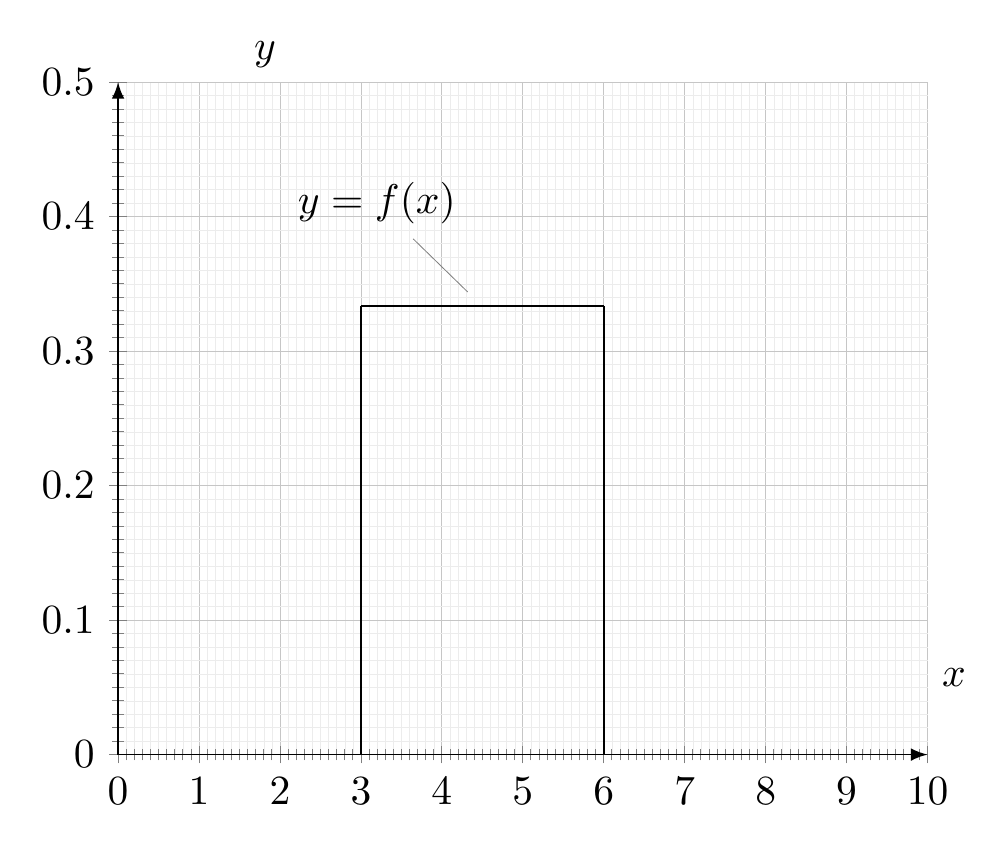
\begin{tikzpicture}[scale=1.5]
		\begin{axis}
			[
			xmin=0,xmax=10,
			ymin=0,ymax=0.5,
			grid=both,
			grid style={line width=.1pt, draw=darkgray!10},
			major grid style={line width=.2pt,draw=darkgray!30},
			axis lines=left,
			minor tick num=9,
			enlargelimits={abs=0},
			axis line style={-latex},
			samples=100,
			domain = -20:20,
			ytick={0,0.1,...,0.5},
			xtick={0,1,...,10},
			xlabel={$x$},
			ylabel={$y$},
			x label style={at={(axis description cs:1,0.15)},anchor=north west},
			y label style={at={(axis description cs:0.15,1)},anchor=south west, rotate=-90}
			]
			
			\addplot [mark=dot] coordinates{(3, 1/3)  (6, 1/3)};
			
			\addplot [mark=dot] coordinates {(3,0) (3, 1/3)};
			
			\addplot [mark=dot] coordinates {(6,1/3) (6,0)};
			
			\node [pin=100:{$y=f(x)$}] at (axis cs:4.5,1/3) {};
		\end{axis}	
	\end{tikzpicture}
	
\end{document}